\section{Đánh giá tư thế ngủ sử dụng cảm biến gia tốc}

% % \subsection{Kiến trúc}
% Hình \ref{tool-architecture} mô tả kiến trúc công cụ được xây dựng theo phương pháp đã được đề xuất ở Chương 3. Cụ thể, công cụ được xây dựng bằng ngôn ngữ Typescript với ba tầng chính là: tầng trình diễn, tầng xử lý lôgic và tầng lưu trữ dữ liệu. Trong đó tầng xử lý lôgic là tầng cốt lõi của công cụ, bao gồm các tác vụ phân tích, tính toán, thực thi nhằm phục vụ cho mục tiêu sinh tập các ca kiểm thử và xuất báo cáo độ phủ tương ứng. Các tác vụ có trong bộ xử lý lôgic tương đương với các giải pháp được hiện thực hóa trong Chương 3, bao gồm thành phần sinh AST, thành phần sinh CFG, thành phần sinh đường kiểm thử, thành phần thực thi tượng trưng, thành phần sinh tệp kiểm thử và thành phần thực thi mã nguồn.
% \begin{itemize}
%     \item Thành phần sinh AST (AST Generation): Mô-đun phân tích mã nguồn thành cây cú pháp trừu tượng. Trong bước này, công cụ sử dụng thư viện có sẵn là ``ts-morph'' được phát triển và mở rộng từ trình biên dịch TypeScript. Các thành phần trong AST có đầy đủ tất cả các phương thức để trích xuất thông tin cần thiết hỗ trợ cho các giai đoạn tiếp theo.
%     \item Thành phần sinh CFG (CFG Generation): Mô-đun đảm nhiệm tác vụ sinh CFG cho một hàm được lựa chọn để sinh dữ liệu kiểm thử. Đầu vào của mô-đun là AST tương ứng với hàm. Dữ liệu này có được từ thư viện phân tích mã nguồn TypeScript ``ts-morph''. Với một hàm bất kỳ, cây cấu trúc trừu tượng của hàm được mô tả bằng lớp \textit{FunctionDeclaration}. Đây là cấu trúc dữ liệu trình biên dịch lưu trữ tất cả các thông tin của thành phần là hàm có trong mã nguồn TypeScript. Các đối tượng kiểu \textit{FunctionDeclaration} đều có phương thức \textit{getStatements()} trả về danh sách các câu lệnh/khối câu lệnh có trong nội dung thân hàm. Mỗi kiểu câu lệnh/ khối câu lệnh có trong mã nguồn được đại diện bằng một lớp. Từ những phương thức được cung cấp bởi lớp đại diện cho mỗi kiểu câu lệnh/khối câu lệnh, thuật toán xây dựng CFG mô tả trong Algorithm \ref{generate-cfg_alg} được cài đặt lại trong lớp \textit{CFGGeneration} trong mã nguồn phát triển công cụ. Lớp này có độ lớn gần 300 dòng mã nguồn, bao gồm phương thức chính là \textit{parse(functionNode: FunctionDeclaration)} cài đặt thuật toán Algorithm \ref{generate-cfg_alg} và một số những phương thức khác hỗ trợ các tác vụ liên quan. Đầu ra của mô-đun này là đối tượng thuộc lớp \textit{CFG} lưu trữ các thông tin cần thiết cho đồ thị dòng điều khiển của một hàm bất kỳ.
%     \item Thành phần sinh đường kiểm thử (Test Path Generation): Mô-đun thực hiện nhiệm vụ thu thập tất cả các đường đi có trong CFG. Sử dụng đối tượng thuộc lớp \textit{CFG} được trả về từ mô-đun sinh CFG trước đó, thuật toán Algorithm \ref{generate-testpath-alg} được cài đặt lại trong phương thức \textit{traverseCFG()} của lớp \textit{TestpathGeneration} như trong Hình \ref{CfgElement}. Phương thức có độ dài khoảng 50 dòng lệnh, bao gồm các thao tác thêm phần tử vào cấu trúc dữ liệu lưu trữ đường đi, lời gọi đệ quy tới các đỉnh tiếp theo và đánh dấu nhánh rẽ của các đỉnh điều kiện. Đầu ra của giai đoạn này là một danh sách bao gồm tất cả những đường đi có thể có của hàm kiểm thử. 
%     \item Thành phần thực thi tượng trưng (Symbolic Execution): Mô-đun này cũng được cài đặt thủ công bằng thuật toán được mô tả trong Algorithm \ref{symbolic-execution}. Các lớp thiết kế sử dụng chính để xây dựng trong phần này đã được mô tả trong Hình \ref{symbolic-expression}. Đây là bước vô cùng quan trọng ảnh hưởng đến độ phủ có thể đạt được của bộ dữ liệu kiểm thử. Quá trình thực thi tượng trưng cần bao phủ được nhiều nhất có thể các hình thức khác nhau của mã nguồn. Điều này giúp cho việc mô tả các biểu thức ràng buộc của các đỉnh điều kiện chính xác hơn. Từ đó, nghiệm của hệ ràng buộc có thể đảm bảo chắc chắn đường đi tương ứng được thực thi trong môi trường thật. Hiện tại, mô-đun này đã xử lý được các biểu thức giá trị là các phép toán +,-,*,/ với các biến có kiểu dữ liệu là số nguyên. Ngoài ra, biểu thức có thể sử dụng một số phương thức/thuộc tính của biến kiểu dữ liệu \textit{string} như \textit{length, startsWith(), includes(), endsWith()}. Đối với các mã lệnh truy cập phần tử mảng, thuộc tính hoặc phương thức của đối tượng, các biến mới được khởi tạo trong bảng \textit{SymbolicTable} và đóng vai trò như là một tham số của hàm. Các biến này sẽ được tái cấu trúc, gộp lại thành một tham số có kiểu đối tượng phù hợp với danh sách tham số ban đầu của hàm.
%     % Hiện tại, các hình thức mã nguồn công cụ có thể phân tích và thực thi tượng trưng được liệt kê trong Bảng \ref{table:expressions}.
%     \item Thành phần sinh dữ liệu kiểm thử (Test Data Generation): Mô-đun này sử dụng bộ giải Z3 Theorem Prover để tìm nghiệm cho hệ ràng buộc ứng với mỗi đường đi. Các ràng buộc được cài đặt phương thức chuyển đổi sang chuẩn của bộ giải Z3. Thời gian xử lý phụ thuộc vào độ phức tạp của hệ ràng buộc. Tác vụ này được triển khai bằng cách tạo một tiến trình con trong hệ điều hành và thực thi câu lệnh \textit{z3 -smt2 <constraint file name>.smt2} để thực hiện quá trình giải hệ. Để quá trình giải quyết các tác vụ liên quan đến bất đồng bộ được chính xác, công cụ sử dụng API của NodeJS đó là \textit{child\_proccess}. Tiến trình con được khởi tạo và thực thi bằng hàm \textit{spawnSync(<câu lệnh>)}. Hàm này đảm bảo tiến trình giải hệ kết thúc mới chuyển sang các tác vụ tiếp theo. Đối tượng trả về của hàm có thuộc tính \textit{stdout} chứa kết quả sau khi giải hệ. Công cụ sử dụng thông tin này để phân tích và chuyển đổi thành đầu vào hợp lệ cho các ca kiểm thử.
%     % \item Thành phần sinh tệp kiểm thử (Test Script Generation): Do tệp kiểm thử có các ca kiểm thử được triển khai bằng các mã lệnh tương đồng với nhau về mặt thứ tự nên hiện tại trong khóa luận này, tệp kiểm thử được hoàn thiện bằng cách chèn lần lượt các dòng lệnh thỏa mãn cú pháp của trình biên dịch. Các dòng lệnh này có nhiệm vụ khởi tạo danh sách tham số từ các ca kiểm thử được sinh ra, tạo thực thể lớp từ JSON, gọi hàm với tham số hợp lệ. Trong giai đoạn phát triển tiếp theo, quá trình này có thể được thay thế bằng giải pháp tối ưu hơn.
%      \item Thành phần sinh và thực thi tệp kiểm thử (Test Script Generation and Execution): Do tệp kiểm thử có các ca kiểm thử được triển khai bằng các mã lệnh tương đồng với nhau về mặt thứ tự nên hiện tại trong khóa luận này, tệp kiểm thử được hoàn thiện bằng cách chèn lần lượt các dòng lệnh thỏa mãn cú pháp của trình biên dịch. Các dòng lệnh này có nhiệm vụ khởi tạo danh sách tham số từ các ca kiểm thử được sinh ra, tạo thực thể lớp từ JSON, gọi hàm với tham số hợp lệ. Trong giai đoạn phát triển tiếp theo, quá trình này có thể được thay thế bằng giải pháp tối ưu hơn. Để thực thi tệp kiểm thử, công cụ sử dụng sự hỗ trợ của Mocha và Istanbul, gọi lệnh \textit{npm install} để cài đặt thư viện sử dụng và gọi lệnh \textit{nyc mocha} để chạy tệp kiểm thử, xuất báo cáo độ phủ.
%     % \item Thành phần thực thi (Test Script Execution): Trong phần này, công cụ sử dụng sự hỗ trợ của Mocha và Istanbul, gọi lệnh \textit{npm install} để cài đặt thư viện sử dụng và gọi lệnh \textit{nyc mocha} để chạy tệp kiểm thử, xuất báo cáo độ phủ.
% \end{itemize} 

% Tầng trình diễn của công cụ được phát triển bằng ngôn ngữ React. Màn hình bắt đầu cho phép người dùng tải lên mã nguồn của dự án dưới dạng tệp zip như Hình \ref{upload-screen}. Ngoài ra, người dùng cần thiết lập đường dẫn tới thư mục mã nguồn gốc của dự án tại trường \textit{Source Root Directory}. Sau đó công cụ sẽ giải nén và phân tích mã nguồn để trả về cấu trúc dự án dưới dạng cây thư mục như Hình \ref{tree-folder}. Tại màn hình cấu trúc mã nguồn dự án, người sử dụng có thể chọn danh sách các hàm cần sinh dữ liệu kiểm thử, sau đó chọn nút ``Generate'' để sinh các ca kiểm thử và tệp kiểm thử tương ứng. Để chạy các tệp kiểm thử, người dùng thao tác với nút \textit{Run test script}.  Quá trình này cũng xuất ra báo cáo về độ phủ của bộ dữ liệu kiểm thử vừa sinh ra dưới dạng HTML như Hình \ref{coverage-report}. Cuối cùng, tầng dữ liệu được xây dựng nhằm mục đích lưu trữ các dữ liệu cần thiết phục vụ quá trình quản lý mã nguồn, lịch sử phân tích, v.v. Trong giai đoạn phát triển hiện tại, công cụ chưa sử dụng đến tầng này vì hiện chưa có chức năng nào cần lưu trữ dữ liệu.

% \begin{figure}[!ht]
% 		\centering
%  		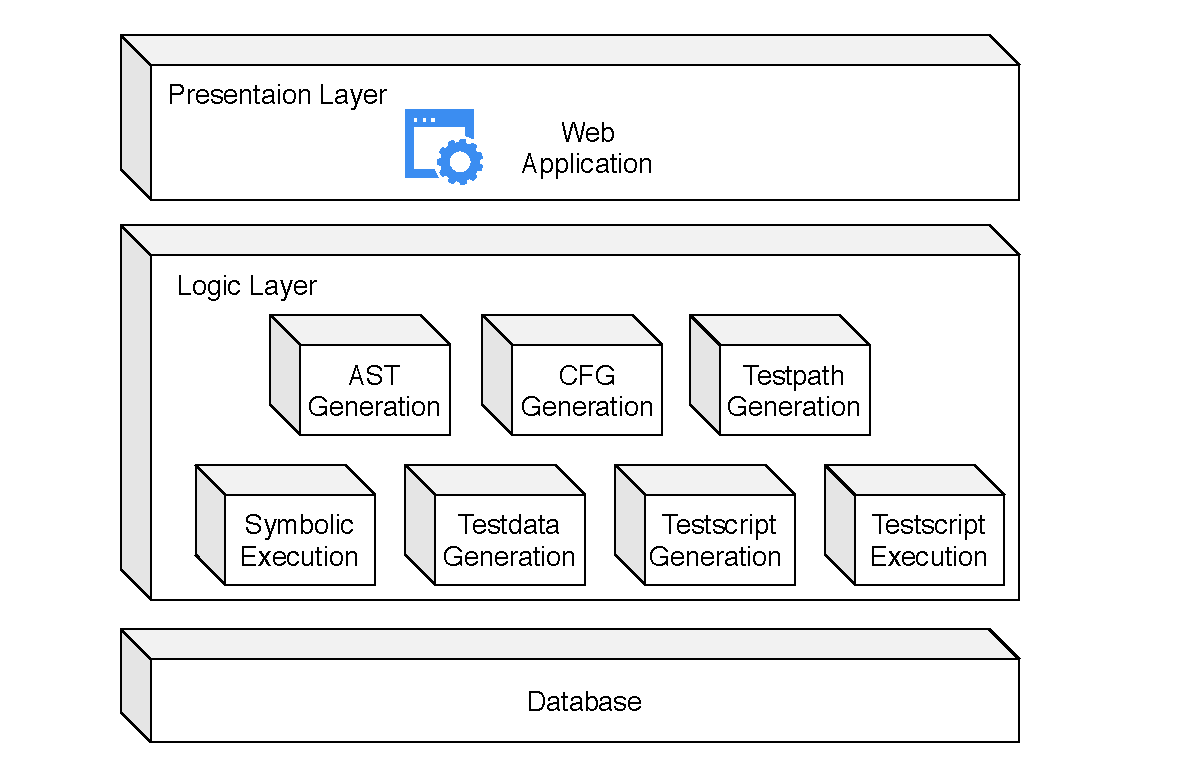
\includegraphics[width=\textwidth]{images/Architecture-Layer.pdf}
%  		\vspace{-1cm}
% 		\caption{Kiến trúc công cụ}
% 		\label{tool-architecture}
% \end{figure}

% \begin{figure}[!ht]
% 		\centering
%  		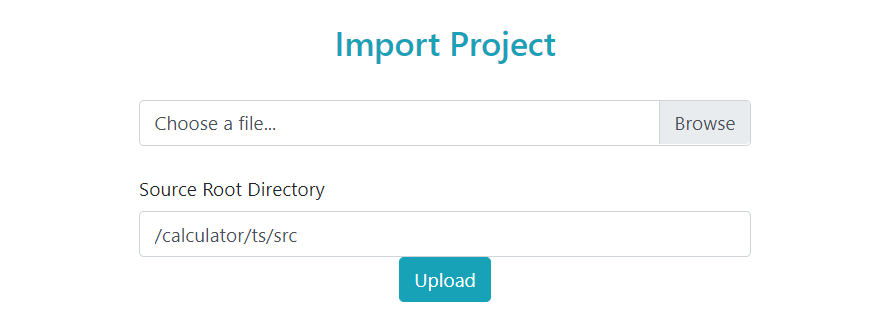
\includegraphics[width=\textwidth]{images/upload-screen.png}
%  		\vspace{-0.7cm}
% 		\caption{Màn hình tải lên mã nguồn dự án}
% 		\label{upload-screen}
% \end{figure}

% \begin{figure}[!ht]
% 		\centering
% 		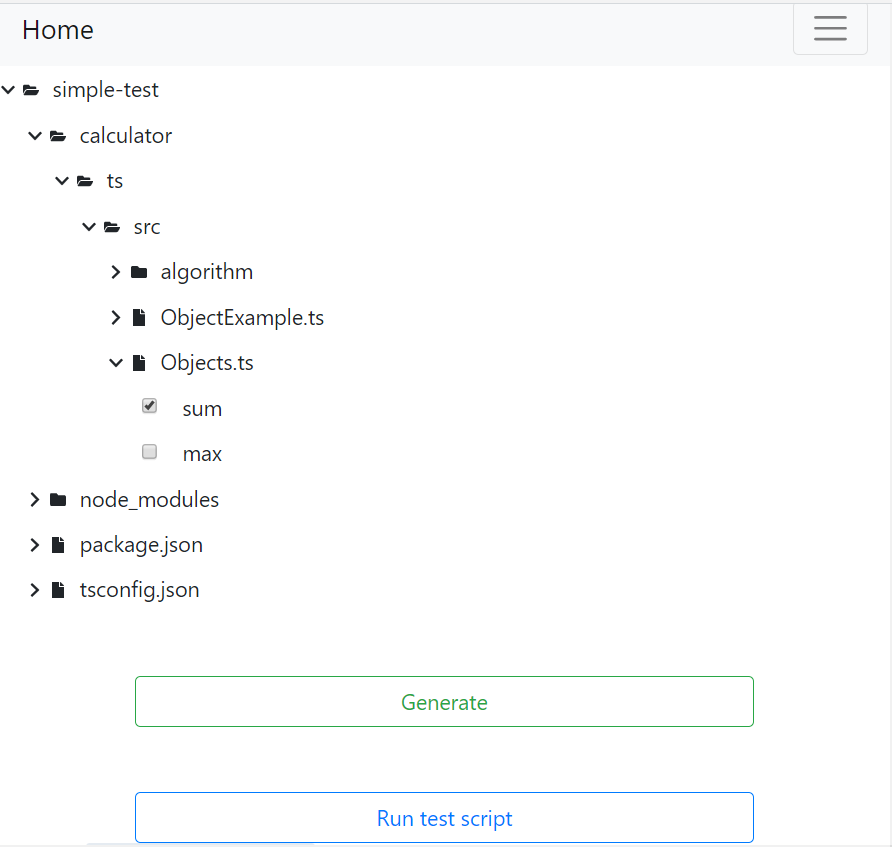
\includegraphics[width=\textwidth]{images/tree-folder.png}
% 		\caption{Màn hình cấu trúc thư mục mã nguồn dự án}
% 		\label{tree-folder}
% \end{figure}

% \begin{figure}[!ht]
% 		\centering
%  		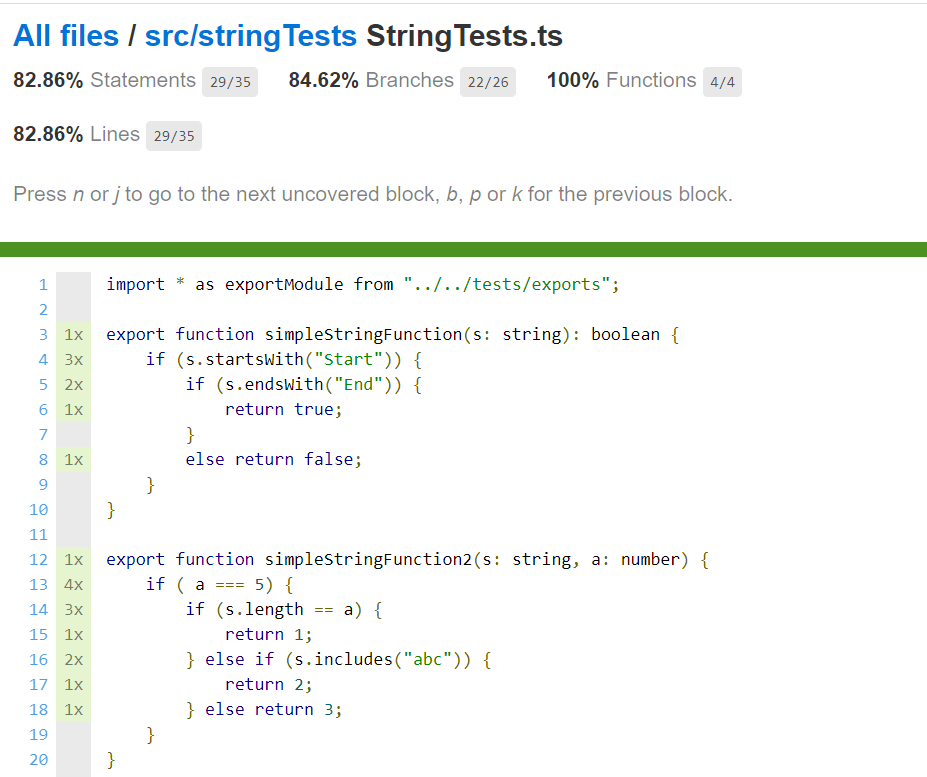
\includegraphics[width=\textwidth]{images/coverage-report.png}
% 		\caption{Ví dụ báo cáo độ phủ được sinh bởi Istanbul}
% 		\label{coverage-report}
% \end{figure}
% % Tầng nghiệp vụ là tầng kết nối giữa tầng trình diễn và tầng xử lý lôgic. Với mỗi yêu cầu từ tầng trình diễn gọi đến một API, tầng nghiệp vụ sẽ gọi dịch vụ từ tầng xử lý lôgic tương ứng.
% % Cuối cùng, tầng dữ liệu được xây dựng nhằm mục đích lưu trữ các dữ liệu cần thiết phục vụ quá trình quản lý mã nguồn, lịch sử phân tích, v.v. Trong giai đoạn phát triển hiện tại, công cụ chưa sử dụng đến tầng này vì hiện chưa có chức năng nào cần lưu trữ dữ liệu.
% % Công cụ sử dụng trinh biên dịch TypeScript để phân tích mã nguồn, bộ giải Z3 để giải hệ ràng buộc, Mocha để chạy test và sinh báo cáo dưới dạng HTML bằng thư viện Istanbul. Công cụ được phát triển bằng chính ngôn ngữ TypeScript, xây dựng CFG và sinh bộ dữ liệu kiểm thử có độ phủ nhánh cao. Hiện nay, công cụ vẫn đang trong thời gian phát triển hoàn thiện hơn để có thể xử lý thêm các trường hợp phức tạp, nâng cao độ phủ và có thể sử dụng thật trong quy trình phát triển phần mềm của doanh nghiệp.

% % \subsection{Đầu vào của công cụ}
% % Công cụ nhận đầu vào là mã nguồn của dự án viết bằng ngôn ngữ TypeScript. Sau khi lưu trữ file và phân tích, cấu trúc mã nguồn được hiển thị dưới dạng cây thư mục. Đối với mỗi tệp mã nguồn, giao diện cũng hiển thị danh sách các hàm có trong tệp đó. Người dùng có thể lựa chọn danh sách các hàm cần được sinh dữ liệu kiểm thử. 
% % Hiện tại, công cụ có thể sinh dữ liệu kiểm thử cho các hàm có tham số đầu vào là number, string, boolean, object, array. Nội dung hàm bao gồm các câu lệnh rẽ nhánh, khai báo biến, gán giá trị cơ bản. Các dạng câu lệnh như vòng lặp, câu điều kiện rút gọn,v.v. sẽ được xử lý trong giai đoạn phát triển tiếp theo.

% % \textbf{Source \ref{lst:inputexample}} là ví dụ một hàm mà công cụ có thể sinh dữ liệu kiểm thử phủ tất cả các nhánh.

% % \begin{lstlisting}[caption=Ví dụ đầu vào, label=lst:inputexample,language=ES6, captionpos=b] 
% % export function caculate2(isBig: boolean, person: Person): number {
% %     let result = person.age + person.height;
% %     let x : boolean = true;
% %     let y;
% %     y = 1;
% %     y = isBig;
% %     if (person.age == 18 && person.school.numberRoom > 30) {
% %         if (person.height > 10 && y != true) {
% %             return 1;
% %         }
% %         else return 2;
% %     }
% %     return result;
% % }
% % \end{lstlisting}

% % \subsection{Đầu ra của công cụ}
% % \subsubsection{Tệp kiểm thử}
% % Khóa luận sử dụng bộ giải Z3 để giải hệ ràng buộc, chuẩn hóa nghiệm của hệ trở thành giá trị truyền vào ham như là một tham số hợp lệ đầy đủ các thuộc tính, hành vi của lớp tương ứng. Từ các bộ giá trị này, tệp kiểm thử được sinh tự động sao cho thỏa mãn cú pháp của Mocha, không bị lỗi biến dịch, đường kiểm thử dùng để sinh dữ liệu thực sự được chạy qua trong môi trường thật. Source \ref{lst:script-example} là một ví dụ cho tệp kiểm thử được sinh tự động.

% % \begin{lstlisting} [caption=Ví dụ tệp kiểm thử hợp lệ cho một ca kiểm thử, label=lst:script-example,language=ES6, captionpos=b] 
% % import {external_function_test} from "../../src/externals/ExternalExample";
% % import { SerializationHelper} from "../SerializationHelper";
% % import {ImportMock} from "TypeScript-mock-imporTypeScript";
% % import * as exportModule from "../exporTypeScript";
% % describe("Test",  () => {
% %     it("Test",  () => {
% %         const stub1 = ImportMock.mockFunction(exportModule, 'max', 4);
% %         const stub2 = ImportMock.mockFunction(exportModule, 'sum', 4);
% %         const mockManager1 = ImportMock.mockStaticClass(exportModule, "Algorithm");
% %         mockManager1.mock("max", 9);
% %         mockManager1.mock("sum", 7);
% %         const object =   {"a":5,"b":6};
% %         let paramters: any = {};
% %         SerializationHelper.fillFromJSON(JSON.stringify(object), paramters);
% %         external_function_test.apply(null, [paramters["a"],paramters["b"],]);
% %         ImportMock.restore();
% %     });
% % });
% % \end{lstlisting}

% % % \begin{figure}[!ht]
% % % 		\centering
% % %  		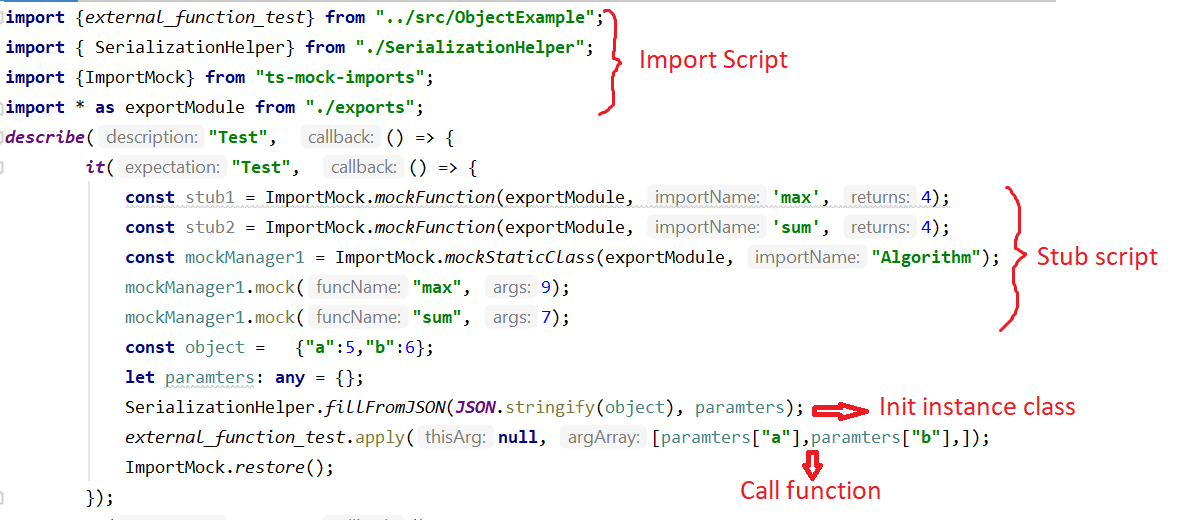
\includegraphics[width=\textwidth]{images/scriptgeneration.png}
% % % 		\caption{Ví dụ tệp kiểm thử hợp lệ cho một testcase}
% % % 		\label{script-example}
% % % \end{figure}

% % \subsubsection{Báo cáo độ phủ}
% % Sau khi thực thi tệp kiểm thử, công cụ xuất ra báo cáo về độ phủ dưới dạng HTML nhờ thư viện Istanbul. Các độ phủ được tính bao gồm có phủ statemenTypeScript, phủ branches, phủ functions, phủ lines. Ngoài ra, báo cáo còn làm nổi bật những dòng lệnh không được chạy qua. HÌnh \ref{coverage-report} là ví dụ về một tệp báo cáo độ phủ dưới dạng HTML được xuất ra bởi Istanbul. Trong đó, tệp mã nguồn \textit{stringTesTypeScript.ts} đạt các độ đo kiểm thử là:  phủ 82.86\% câu lệnh, phủ 84.62\% các nhánh có trong tệp, phủ 100\% functions nghĩa là tất cả các hàm có trong tệp đều được gọi ít nhất 1 lần.

% % \begin{figure}[!ht]
% % 		\centering
% %  		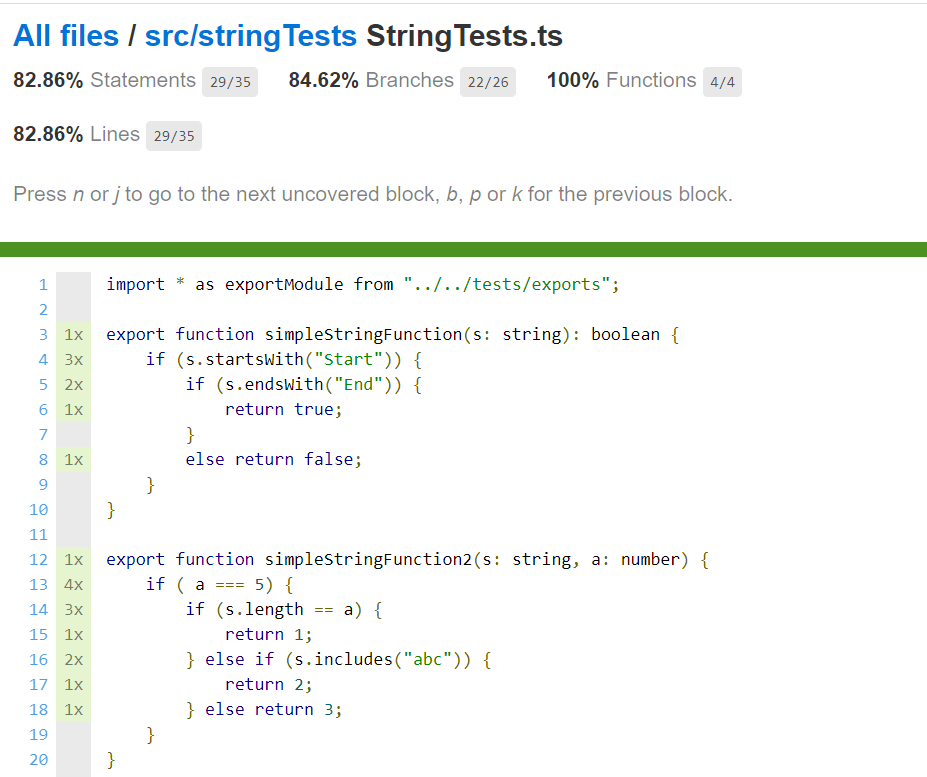
\includegraphics[width=\textwidth]{images/coverage-report.png}
% % 		\caption{Ví dụ báo cáo độ phủ được sinh bởi Istanbul}
% % 		\label{coverage-report}
% % \end{figure}

% \section{Ví dụ minh họa}
% Để mô tả rõ hơn những tính năng của công cụ, nội dung của phần này trình bày một ví dụ sinh dữ liệu kiểm thử đơn vị cho một tệp mã nguồn TypeScript. Đầu vào là một mã nguồn TypeScript\footnote{\url{https://github.com/doanthihoaithu/typescript-project-examples}} bao gồm các hàm đơn giản tương ứng với các trường hợp tham số kiểu khác nhau. Nội dung các hàm này bao gồm các lệnh khai báo biến, lệnh gán và câu lệnh điều kiện rẽ nhánh. Thư mục mã nguồn chính của ví dụ là \textit{calculate/ts/src}\footnote{\url{https://github.com/doanthihoaithu/typescript-project-examples/tree/master/calculator/ts/src}}. Đường dẫn của đến thư mục này cần được người dùng thiết lập trước khi tải lên mã nguồn dự án. Các thao tác phân tích xử lý sẽ được thực hiện trên các tệp mã nguồn có trong thư mục này. Dữ liệu các ca kiểm thử của các hàm được lựa chọn để kiểm thử được lưu trong thư mục \textit{calculate/ts/testdata\_dtht}\footnote{\url{https://github.com/doanthihoaithu/typescript-project-examples/tree/master/calculator/ts/testdata\_dtht}}. Tập các ca kiểm thử của một hàm được lưu trữ dưới dạng JSON trong tệp có đường dẫn tương đương với đường dẫn của hàm đó trong thư mục mã nguồn chính. Dữ liệu này được sử dụng lại trong quá trình sinh tệp kiểm thử. Thư mục lưu trữ các tệp kiểm thử là \textit{calculate/ts/tests}\footnote{\url{https://github.com/doanthihoaithu/typescript-project-examples/tree/master/calculator/TypeScript/tests}}. Mỗi tệp mã nguồn trong thư mục này tương ứng với một hàm được chọn để sinh dữ liệu kiểm thử. Các tệp này có tên kết thúc bằng chuỗi \textit{.test.ts} nhằm đánh dấu đây là những tệp kiểm thử để công cụ Mocha có thể thực thi một cách chính xác. Thư mục \textit{images}\footnote{\url{https://github.com/doanthihoaithu/typescript-project-examples/images}} lưu trữ một số hình ảnh liên quan đến giao diện của công cụ. Hình \ref{selectFunction} mô tả giao diện màn hình cấu trúc mã nguồn, bao gồm thành phần hiển thị cấu trúc và thành phần hiển thị nội dung của mã nguồn. Đối với thành phần hiển thị cấu trúc thư mục, công cụ hỗ trợ chức năng lựa chọn hàm để sinh tập kiểm thử. Về thành phần hiển thị nội dung, giao diện hiển thị như một màn hình soạn thảo mã nguồn. Người dùng cũng có thể thực hiện thao tác thay đổi nội dung đối với một tệp bất kỳ. Với các tệp là mã nguồn TypeScript, giao diện cấu trúc mã nguồn dưới dạng cây thư mục cũng hiển thị danh sách các hàm có trong tệp đó để người dùng có thể lựa chọn cho quá trình kiểm thử. Với mỗi tệp TypeScript được chọn, nội dung của tệp sẽ được hiển thị tại phần chính giữa màn hình. Sau khi chọn nút \textit{Generate}, công cụ bắt đầu thực hiện tác vụ sinh dữ liệu kiểm thử tự động. Tập ca kiểm thử được lưu trong thư mục \textit{calculator/ts/testdata\_dtht}. Nội dung của các tệp này được hiển thị ở bên trái màn hình tương ứng với hàm mà kỹ thuật viên lựa chọn tại cây thư mục. Hình \ref{abs-testcases} liệt kê các ca kiểm thử được sinh tự động bởi công cụ cho hàm \textit{abs()} trong tệp \textit{Utils.ts}\footnote{\url{https://github.com/doanthihoaithu/typescript-project-examples/blob/master/calculator/ts/src/algorithm/Utils.ts}}. Trong đó, có tất cả ba ca kiểm thử ứng với ba đường đi của hàm \textit{abs()}. Kết quả cho thấy $a=\{1, -1, 0\}$ là tập ca kiểm tử được sinh tự động cho hàm này với độ phủ đạt được là 100\%.

% \begin{figure}[!ht]
% 		\centering
% 		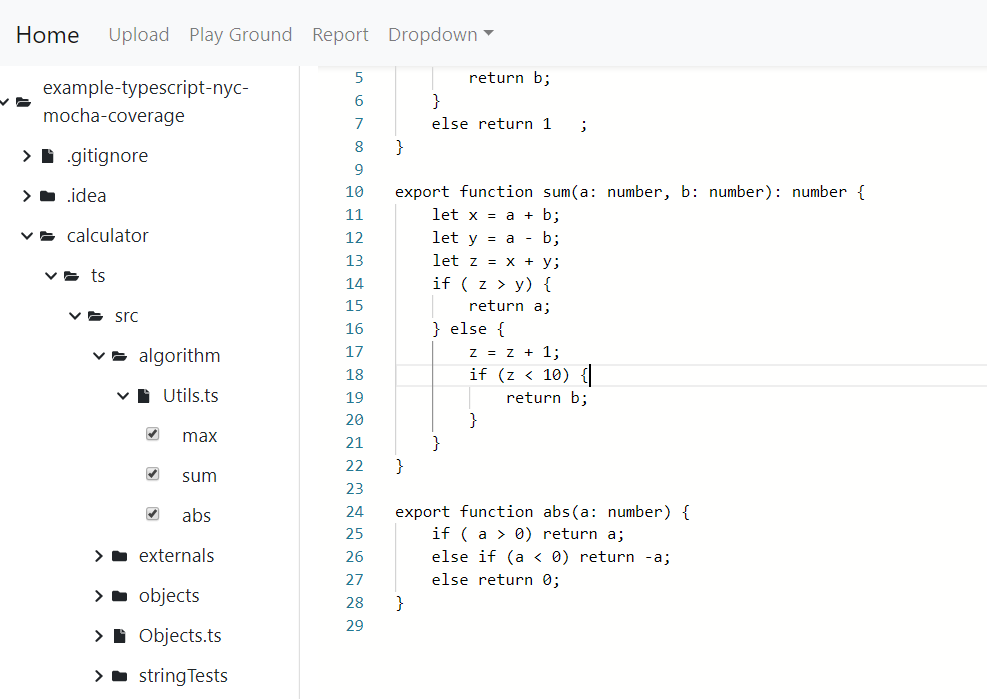
\includegraphics[width=\textwidth]{images/selectFunctionExample.png}
% 		\caption{Màn hình lựa chọn hàm sinh tập kiểm thử}
% 		\label{selectFunction}
% \end{figure}

% \begin{figure}[!ht]
% 		\centering
% 		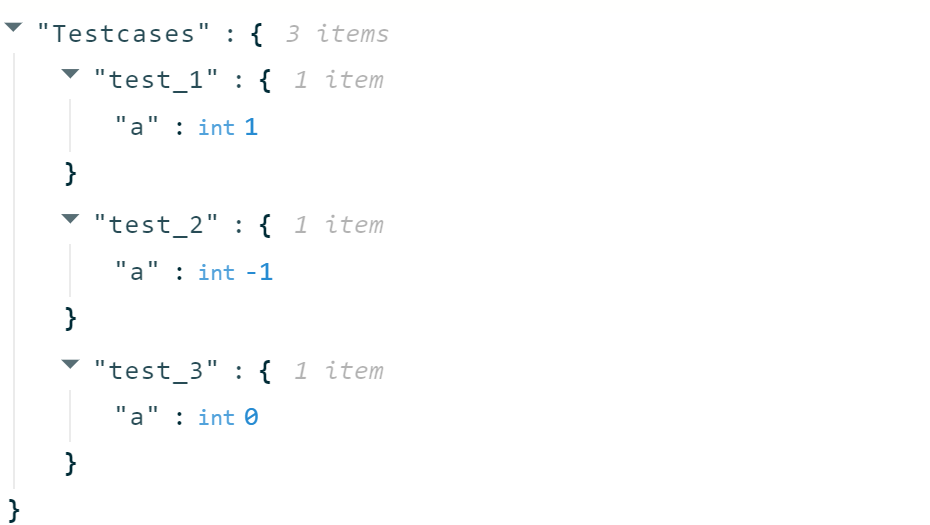
\includegraphics[width=13cm]{images/testcases.png}
% 		\caption{Màn hình danh sách ca kiểm thử cho hàm \textit{abs()}}
% 		\label{abs-testcases}
% \end{figure}

% Hình \ref{coverageOfExampleProject} là báo cáo độ phủ khi tất cả các hàm có trong ví dụ minh họa được lựa chọn để sinh dữ liệu kiểm thử. Tỉ lệ các độ phủ của các thư mục được thể hiện bằng số liệu tại các cột Statements, Branches, Functions, Lines. Các tiêu chí độ phủ nếu đạt 100\% được phủ màu xanh, đạt tỉ lệ trung bình được phủ màu vàng. Nếu tỉ lệ độ phủ của tệp dưới mức cảnh báo thì các ô số liệu của thư mục/tệp này được phủ màu đỏ. Ranh giới giữa các mức độ bao phủ tốt, trung bình, thấp có thể được thiết lập bởi kỹ thuật viên.

% \begin{figure}[!ht]
% 		\centering
% 		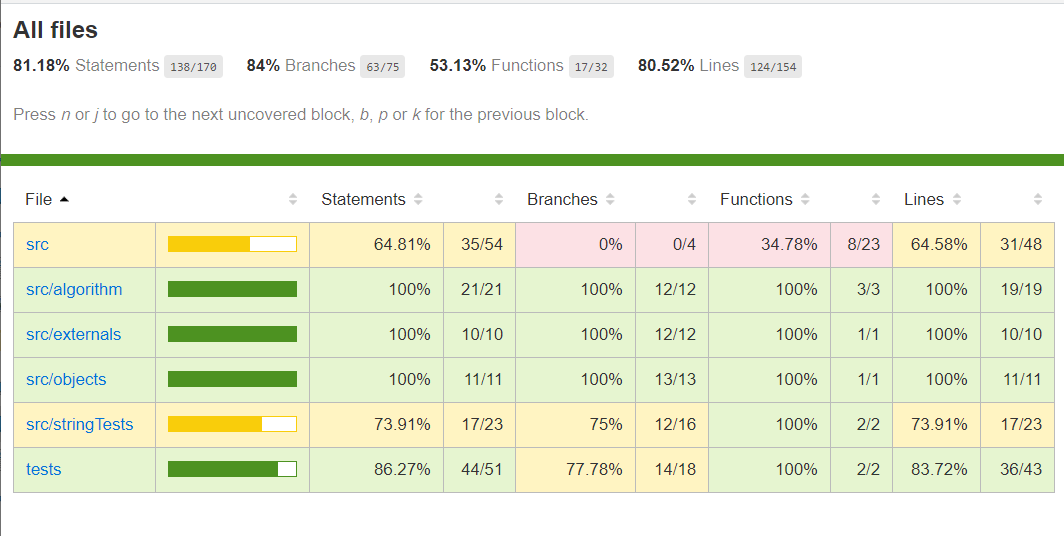
\includegraphics[width=\textwidth]{images/coverageOfExampleProject.png}
 		
% 		\caption{Màn hình báo cáo độ phủ}
% 		\label{coverageOfExampleProject}
% \end{figure}

% \section{Thực nghiệm}
% Để chỉ ra tính hiệu quả của công cụ được xây dựng, phần thực nghiệm sử dụng công cụ để sinh dữ liệu kiểm thử cho một mã nguồn TypeScript\footnote{\url{https://github.com/doanthihoaithu/applied-ts-project}}. Nội dung mã nguồn bao gồm nhiều tệp mã nguồn TypeScript. Mỗi tệp có nhiều hàm thực hiện chức năng tính toán độc lập. Tham số đầu vào có kiểu dữ liệu đa dạng, bao gồm kiểu dữ liệu nguyên thủy, mảng và đối tượng. Mã nguồn được chia thành bốn nhóm theo đặc trưng của kiểu tham số đầu vào và các biến được sử dụng trong hàm. Thư mục \textit{algorithm} bao gồm các hàm có tham số đầu vào thuộc kiểu dữ liệu nguyên thủy. Thư mục \textit{stringTests} bao gồm các hàm có tham số thuộc kiểu dữ liệu \textit{string} và nội dung hàm sử dụng các phương thức mặc định của kiểu dữ liệu này. Thư mục \textit{objects} bao gồm các hàm có tham số đầu vào thuộc kiểu dữ liệu phức tạp hơn như mảng hoặc đối tượng. Còn các hàm có sử dụng lời gọi hàm bên ngoài được lưu trữ trong thư mục \textit{externals}.  Bảng \ref{table:appliedProject} thống kê  các kết quả kiểm thử được đo đạc trong quá trình tiến hành thực  nghiệm, bao gồm số lượng dòng lệnh của tệp kiểm thử, số ca kiểm thử sinh được, độ bao phủ nhánh và chi phí thời gian tương ứng. Số lượng các dòng lệnh có trong tệp (Line of Code - LOC) được đo đạc bởi công cụ LocMetrics\footnote{http://www.locmetrics.com/}. Về độ phủ nhánh, số liệu của cột này được lấy ra trong báo cáo độ phủ được sinh ra nhờ thư viện Istanbul. Thử nghiệm được thực hiện với máy tính cài đặt hệ điều hành Window có cấu hình 8G Ram, bộ xử lý Intel(R) Core(TM) i5-8250U CPU @ 1.60Ghz.

% \begin{table}[h!]
%     \centering
%     \caption{Bảng thống kê kết quả kiểm thử theo tệp}
%     \vspace{0.5cm}
%     \begin{adjustbox}{width=1\textwidth}
%     \small
%     \begin{tabular}{ |p{0.7cm}|p{5.3cm}|p{2cm}|p{2cm}|p{2cm}|p{2cm}| }
%          \hline
%          \textbf{STT} & \textbf{Tệp}  & \textbf{LOC}  & \textbf{Số ca kiểm thử} & \textbf{Độ phủ nhánh} & \textbf{Thời gian (ms)}\\
%          \hline
%          1 & algorithm/Abs.ts &  6 &  3 &  100\% &  448 \\
%         \hline
%          2 & algorithm/BooleanTest.ts &  9 &  3 &  100\% &  411 \\
%         \hline
%          3 & algorithm/CalculateDiscount.ts &  18 &  5 &  100\% &  516 \\
%         \hline
%          4 & algorithm/Loop.ts &  18 &  2 &   66.67\% &  449 \\
%         \hline
%          5 & algorithm/Max.ts &  9 &  3 &  100\% &  394 \\
%         \hline
%          6 & algorithm/Sum.ts &  14 &  3 &  100\% &  417 \\
%         \hline
%          7 & externals/ExternalExample.ts &  16 &  4 &  100\% &  654 \\
%         \hline
%          8 & stringTests/StringParam1.ts &  9 &  3 &  100\% &  444 \\
%         \hline
%          9 & stringTests/StringParam2.ts &  10 &  4 &  100\% &  388 \\
%         \hline
%          10 & stringTests/StringParam3.ts &  14 &  5 &  100\% &  540 \\
%         \hline
%          11 & stringTests/StringParam4.ts &  18 &  4 &  50\% &  600 \\
%         \hline
%          12 & objects/ObjectParam1.ts &  15 &  3 &  100\% &  488 \\
%         \hline
%          13 & objects/ObjectParam2.ts &  15 &  3 &  100\% &  450 \\
%         \hline
%          14 & objects/ObjectParam3.ts &  22 &  3 &  100\% &  430 \\
%         \hline
%          15 & objects/ObjectParam4.ts &  15 &  3 &  100\% &  431 \\
%         \hline
%          16 & objects/ObjectParam5.ts &  16 &  3 &  100\% &  463 \\
%         \hline
%          17 & objects/ObjectParam6.ts &  16 &  4 &  100\% &  525 \\
%         \hline
%          18 & objects/ObjectParam7.ts &  18 &  4 &  100\% &  498 \\
%         \hline
%          19 & objects/ObjectParam8.ts &  16 &  4 &  100\% &  750 \\
%         \hline
%          20 & objects/ObjectParam9.ts &  18 &  3 &  100\% &  499 \\
%         \hline
%          21 & objects/ObjectParam10.ts &  15 &  3 &  100\% &  466 \\
%         \hline
%         % StringProperty SymExpression   & "str.len " + identifier.toZ3Text()\\
%         % \hline
%         % StringMethod SymbolicExpression &  "str.prefixof "+ argumentName + " " + identifier.toZ3Text();\\
%         % \hline
%         % Binary SymbolicExpression&  operator + " " + left.toZ3Text() + " " + right.toZ3Text()\\
%         % \hline
%         % PrefixUnary SymbolicExpression& not + " " + expression.toZ3Text()\\
%         % \hline
%         % Initialized SymbolicExpression   & Không thay đổi\\
%         \end{tabular}
%     \end{adjustbox}
%     \label{table:appliedProject}
% \end{table}

% Trong Bảng \ref{table:appliedProject}, đối với các hàm sử dụng kiểu tham số nguyên thủy như \textit{boolean}, \textit{number} hoặc \textit{string} có trong thư mục \textit{algorithm} và \textit{stringTests}, bộ dữ liệu kiểm thử được sinh tự động có thể đạt được độ phủ 100\%. Công cụ cũng có thể xử lý các cú pháp truy cập thuộc tính của đối tượng hoặc truy cập phần tử của mảng đa dạng được đề cập đến trong thư mục \textit{object}. Tệp \textit{ExternalExample.ts} là một ví dụ khi nội dung thân hàm có chứa lời gọi đến hai hàm độc lập ngoài tệp này là \textit{Algorithm.max()} và \textit{Algorithm.sum()}. Mỗi hàm này được coi như là một tham số đầu vào với giả thiết là nó có thể nhận bất cứ giá trị nào thuộc miền giá trị của kiểu dữ liệu. Giá trị trả về của hàm để thỏa mãn đường đi tương ứng có trong kết quả giải hệ ràng buộc. Những giá trị này được lưu trữ và sử dụng để thiết lập giá trị trả về mặc định cho chính hàm đó tại tệp kiểm thử. Do đó, khi thực thi thật, hệ ràng buộc của tất cả các đường đi của hàm đều được thỏa mãn. Kết quả là độ bao phủ của hàm kiểm tra vẫn đạt 100\% khi thực thi các tệp kiểm thử.

% Trong trường hợp gặp những câu lệnh chưa được xử lý như vòng \textit{for}, \textit{while}, câu điều kiện rút gọn, v.v. thì tệp chưa đạt được độ phủ tối đa. Trong ví dụ này, tệp  \textit{StringParam4.ts} có hàm sử dụng biểu thức \textit{substring()}. Biểu thức này chưa được phân tích trong bộ xử lý chính của công cụ nên ca kiểm thử sinh ra khi thực thi trong môi trường thật không thỏa mãn đường đi tương ứng với ca kiểm thử. Vì vậy độ phủ nhánh của tệp này chỉ đạt 50\%. Tương tự với tệp \textit{Loop.ts}, trong tệp này có sử dụng câu lệnh vòng lặp \textit{for} chưa được xử lý, ca kiểm thử không thỏa mãn điều kiện của vòng lặp nên khối lệnh này không được chạy qua. Do sự đa dạng của mã nguồn trong thực tế nên việc xử lý triệt để các trường hợp tương tự như vậy rất khó khăn. Quá trình này cần có thời gian để hoàn hiện để có thể thực sự áp dụng được với các dự án trong thực tế.

% Số liệu thời gian có trong Bảng \ref{table:appliedProject} được tính toán khi kỹ thuật viên chỉ lựa chọn duy nhất tệp đó để sinh dữ liệu kiểm thử. Bảng \ref{table:totalStatistic} là số liệu khi thực hiện trên toàn bộ mã nguồn. Trong trường hợp này, chi phí thời gian giảm đi do các thao tác đọc ghi dữ liệu và biên dịch mã nguồn được thực hiện đồng thời. Vì vậy,  thời gian thực hiện trên mỗi thư mục nhỏ hơn rất nhiều so với tổng thời gian thực hiện nếu tách riêng từng tệp trong thư mục. Cột độ phủ nhánh trong Bảng \ref{table:totalStatistic} là độ phủ nhánh tổng hợp của cả thư mục, bao gồm những tệp có độ phủ tối đa hoặc độ phủ thấp. Số liệu trong cột này sẽ nằm giữa khoảng độ phủ lớn nhất và độ phủ nhỏ nhất của các tệp có trong thư mục đó. Thư mục \textit{algorithm} có năm tệp đạt độ phủ nhánh tối đa và một tệp đạt độ phủ nhánh 66.67\% nên độ phủ nhánh trung bình đạt được của thư mục này là 93.33\%. Thư mục \textit{externals} chứa một tệp duy nhất là \textit{ExternalExample.ts} đạt độ phủ nhánh 100\% trong Bảng \ref{table:appliedProject}. Vì vậy, thư mục này cũng đạt độ phủ nhánh 100\% nếu tính trên toàn bộ thư mục. Đối với thư mục \textit{stringTests}, tệp \textit{StringParam4.ts} không đạt độ phủ nhánh tối đa nên độ phủ nhánh tổng hợp của thư mục này là 84.62\%. Đối với thư mục \textit{objects}, các tính độ phủ cũng được áp dụng tương tự với các thư mục trên. Cột \textit{Số ca kiểm thử} bằng tổng tất cả các ca kiểm thử của mỗi tệp có trong thư mục đó.
% \begin{table}[h!]
%     \centering
%     \caption{Bảng thống kê kết quả kiểm thử theo thư mục}
%     \vspace{0.5cm}
%     \begin{adjustbox}{width=1\textwidth}
%     \small
%     \begin{tabular}{ |p{1cm}|p{5cm}|p{2cm}|p{2cm}|p{2cm}|p{2cm}| }
%          \hline
%          \textbf{STT} & \textbf{Thư mục}  & \textbf{LOC}  & \textbf{Số ca kiểm thử} & \textbf{Độ phủ nhánh} & \textbf{Thời gian (ms)}\\
%          \hline
%          1 & algorithm &  74 &  19 &  93.33\% &  938 \\
%         \hline
%          2 & externals &  16 &  4 &  100\% &  496 \\
%          \hline
%           3 & stringTests &  51 &  16 &  84.62\% &  1009 \\
%          \hline
%           4 & objects &  166 &  33 &  100\% &  2029 \\
%          \hline
%         \end{tabular}
%     \end{adjustbox}
%     \label{table:totalStatistic}
% \end{table}

% % \section{Ý nghĩa thực nghiệm}

% Kết quả thực nghiệm cho thấy công cụ đã đem lại một số kết quả nhất định trong việc sinh dữ liệu kiểm thử tự động. Mặc dù đây là công cụ đầu tiên hỗ trợ sinh dữ liệu kiểm thử tự động cho TypeScript, tập ca kiểm thử được sinh ra đem lại độ phủ cao. Công cụ đã có thể hỗ trợ rất nhiều kiểu dữ liệu trong TypeScript từ các kiểu dữ liệu cơ bản như \textit{number, string, boolean} cho đến mảng và đối tượng. Đồng thời,  các loại câu lệnh thường được sử dụng trong mã nguồn cũng đã được phân tích và xử lý như biểu thức truy cập phần tử mảng, biểu thức truy cập thuộc tính của đối tượng, lời gọi hàm từ bên ngoài, v.v. Bảng \ref{table:expressions} liệt kê tất cả các hình thức mã nguồn được công cụ hỗ trợ đến thời điểm hoàn thành khóa luận này. Độ phủ có thể đạt 100\%  nếu tất cả các đường đi CFG của hàm là khả thi và cấu trúc mã nguồn thuộc phạm vi được phân tích như trong Bảng \ref{table:expressions}. Nhờ tận dụng thế mạnh của bộ giải ràng buộc Z3 SMT - Lib, công cụ có thể giải các ràng buộc có chứa phương thức của kiểu dữ liệu \textit{string} như \textit{startsWith(), endsWith()}, v.v. Ngoài ra, các ví dụ về hàm có tham số kiểu đối tượng cho thấy công cụ có khả năng xử lý các biểu thức gán giá trị hoặc biểu thức điều kiện phức tạp kết hợp đa dạng của nhiều biểu thức con. Từ đó cho thấy công cụ đã hỗ trợ tương đối những hình thức mã nguồn thường được sử dụng trong thực tế. Phạm vi này có thể được mở rộng trong giai đoạn phát triển tiếp theo và có thể áp dụng cho các dự án thật với mã nguồn đa dạng và phong phú. 
% % Thêm vào đó, công cụ còn cung cấp một quy trình kiểm thử hoàn thiện để kiểm tra mã nguồn, bao gồm việc sinh tập ca kiểm thử có độ phủ cao, sinh tệp kiểm thử, thực thi và xuất báo cáo. Báo cáo độ phủ được hiển thị trực quan, nổi bật những nhánh và dòng mã nguồn không được thực thi. Từ đó, kỹ thuật viên có thể bổ sung ca kiểm thử thủ công hoặc kiểm tra lại tính đúng đắn của mã nguồn. Độ phủ của tập ca kiểm thử có thể tiến dần tới 100\%, có độ tin cậy cao hơn.
% \setlength\LTleft{0pt}
% \setlength\LTright{0pt}
% \setlength\LTcapwidth{\linewidth}
% \begin{longtable}{ |p{1cm}|p{7cm}|p{6,5cm}|}
% % \begin{longtable}{ @{\extracolsep{\fill}}|p{1cm}|p{6,5cm}|p{6,5cm}|@{}}
%     % \centering
%     \caption{Bảng danh sách các dạng biểu thức được hỗ trợ trong mã nguồn}
%     % \vspace{0.5cm}
%     % \begin{adjustbox}{width=1\textwidth}
%     % \small
%     % \begin{tabular}{ |p{1cm}|p{6,5cm}|p{6,5cm}|  }
%     \\
%          \hline
%          \textbf{STT} & \textbf{Kiểu biểu thức} & \textbf{Ví dụ minh họa}\\
%          \hline
%          \endhead
%          \hline
%          \endfoot
%         1 & Biểu thức sử dụng các phép toán với biến nguyên thủy & \makecell[l]{ a = 1 + 2;\\
%          a = 3*4/2;\\
%         if (a > 1);\\ if(a > 1 + 2); \\
%         if (a + 1 > 3*4)} 
%         \\
%         \hline
%         2 & Biểu thức sử dụng các phép toán với tên biến.   & \makecell[l]{ a = b + c;\\ a = b*c;\\
%         if (a > b); \\if (a > b+c); \\
%         if (a + b ==  c + d); \\
%         if (a*b != c/d)}
%         \\
%         \hline
%         3 & Biểu thức sử dụng thuộc tính length của biến kiểu string & \makecell[l]{ s = “abcdef”;\\
%         a = s.length;\\
%         if (s.length > 10);\\
%         if(s.length > a+b); \\
%         if (s1.length < s2.length + a);}
%         \\
%         \hline
%         4 & Biểu thức sử dụng phương thức startsWith(), endsWith(), includes() của biến kiểu string & \makecell[l]{ a = s.startsWith(“ABC”); \\
%         a = endsWith(“DEF”);\\
%         if (s.includes(“XYZ”))}
%         \\
%         \hline
%         5 & Gán một chuỗi cụ thể cho biến kiểu string & a = “abcdef”;\\
%         \hline
%         6 & Biểu thức sử dụng các phép toán với thuộc tính của tham số đối tượng   & \makecell[l]{a = person.height + person.age;\\
%         if (person.height > 180)\\
%         if (person.height/person.age <  8)} 
%         \\ 
%         \hline
%         7 & Biểu thức sử dụng các phép toán với các hàm getter của đối tượng & \makecell[l]{s = person.getName();\\
%         if (person.getName().\\startsWith(“hoaithu”))} 
%         \\
%          \hline
%         8 & Biểu thức sử dụng các phép toán với phần tử mảng có chỉ số cụ thể &\makecell[l]{ a = arr[0] + b; \\
%         a[0] = a + b + a[1];} 
%         \\
%          \hline
%         9 & Biểu thức sử dụng lời gọi các hàm bên ngoài trả về giá trị có kiểu dữ liệu nguyên thủy &\makecell[l]{ a = Algorithm.max(1,2) +\\ Algorithm.max(x,y); \\
%         if (b > Algorithm.max(4,5)) \{\\ <khối lệnh>\\ \}} 
%         \\
%          \hline
%         10 & Biểu thức khai báo/gán giá trị là một mảng & a = [1,2,3,4,5,6];\\
%          \hline
%         11 &Biểu thức khai báo/gán giá trị là một đối tượng JSON & \makecell[l]{a= \{height: 180, age: 23, \\school:\{name: “UET”\}\}}\\
%          \hline
%         12 & Biểu thức điều kiện kép bao gồm biều biểu thức điều kiện đơn thỏa mãn các tính chất 1 -> 9 & If (a > b \&\& s.length > 10 \&\& s.startsWith(“ABC”))
%         % \end{tabular}
%     % \end{adjustbox}
%     \label{table:expressions}
% \end{longtable}

% Tuy nhiên, thực nghiệm cũng cho thấy một số hạn chế vẫn tồn tại trong công cụ. Các cấu trúc điều khiển mã nguồn phổ biến vẫn chưa được xử lý như là vòng lặp, khối lệnh \textit{switch}, câu điều kiện rút gọn, lời gọi đệ quy, v.v. Ngoài ra, công cụ vẫn chưa giải quyết trường hợp chỉ số của phần tử trong mảng là biểu thức hay gọi hàm bên ngoài có kiểu trả về phức tạp.  Tỉ lệ độ phủ có thể đạt được phụ thuộc vào khả năng xử lý đầy đủ và chính xác của quá trình thực thi tượng trưng. Trong trường hợp mã nguồn kiểm thử có những dạng mã nguồn nằm ngoài khả năng xử lý, tập dữ liệu kiểm thử có thể cho kết quả bao phủ thấp. Hiện tại, công cụ vẫn chưa phân tích những hàm được gọi từ bên ngoài hoặc phương thức của đối tượng có trong nội dung hàm. Cho nên việc giả lập một giá trị nào đó cho những hàm kiểu này là không phù hợp với thực tế vì giá trị này có thể không nằm trong miền giá trị của hàm. Trong giai đoạn phát triển tiếp theo, các giải pháp khác sẽ được nghiên cứu để giải quyết vấn đề này. Đồng thời, công cụ sẽ được hoàn thiện thêm về phần xử lý để đáp ứng tối đa tính đa dạng của mã nguồn. 

% \section{Thảo luận}
% Với cách thiết kế theo những giải pháp đã được mô tả trong Chương 3, tính đến thời điểm hoàn thành khóa luận này, công cụ đã được phát triển tương đối hoàn thiện và đạt được một số kết quả nhất định. Về ưu điểm, đây là công cụ đầu tiên cung cấp một quy trình hoàn thiện để tự động hóa pha kiểm thử đơn vị dành cho các ứng dụng TypeScript, từ việc sinh dữ liệu kiểm thử, sinh tệp kiểm thử, thực thi và xuất các báo cáo kiểm thử và báo cáo độ phủ. Ngoài ra, công cụ hỗ trợ hầu hết các kiểu tham số phổ biến như kiểu nguyên thủy, mảng, đối tượng. Độ phủ đối với các hàm có nội dung nằm trong phạm vi phân tích đạt được tỉ lệ cao, có thể đạt 100\% bao phủ nhánh và bao phủ câu lệnh. Thêm vào đó, công cụ có khả năng ứng dụng rất cao khi có thể phát triển theo hướng tích hợp thành một tiện ích trong các trình soạn thảo mã nguồn hoặc tích hợp với quy trình kiểm thử tự động như là pha quan trọng và bắt buộc, giúp giảm thiểu thời gian và công sức cho đội ngũ kiểm thử.

% Về nhược điểm, công cụ chưa hỗ trợ tiêu chuẩn bao phủ MC/DC cho các dự án yêu cầu kiểm thử đơn vị chặt chẽ đối với từng biểu thức điều kiện con. Tuy nhiên, vấn đề này chỉ phụ thuộc vào pha sinh CFG, các bước tiếp theo không có sự khác biệt. Vì vậy, điều này có thể được cải thiện dễ dàng trong giai đoạn phát triển tiếp theo bằng cách thay đổi thành phần sinh CFG. Thứ hai, công cụ chưa thử nghiệm được với các dự án thực tế có quy mô lớn để thể hiện khả năng mở rộng và ứng dụng. Do tính đa dạng của mã nguồn, các dự án thực tế bao gồm nhiều cấu trúc dữ liệu phức tạp, cách triển khai mã nguồn rất phong phú. Những trường hợp này không nằm trong phạm vi phân tích của công cụ nên quá trình xử lý dễ dàng gặp lỗi hoặc bộ dữ liệu kiểm thử sinh ra không có độ phủ cao như mong đợi. Việc xử lý triệt để các trường hợp của mã nguồn rất khó khăn. Vì vậy, hướng giải quyết dành cho bài toán này là cho phép kỹ thuật viên bổ sung thêm các ca kiểm thử thủ công cho những đường đi chứa cấu trúc mã nguồn phức tạp nhưng không được chạy qua. Thứ ba, mặc dù các kiểu tham số phổ biến được công cụ hỗ trợ toàn bộ nhưng vẫn có thể gặp một số trường hợp có tham số kiểu khác như \textit{any, tuple, enum, void, null, undefined, never,} v.v. Các kiểu dữ liệu này thường được sử dụng ít hơn so với các kiểu dữ liệu trong phạm vi hỗ trợ, có những tính chất đặc thù. Việc xử lý toàn bộ cần thêm thời gian và cần có phương án thiết kế mã nguồn hợp lý hơn. Nhược điểm thứ tư của công cụ nằm trong bộ xử lý thực thi tượng trưng và sinh dữ liệu kiểm thử. Theo cách thiết kế các lớp và giải pháp được mô tả trong Chương 3 thì gánh nặng tính toán được chuyển sang phía bộ giải Z3. Nếu ràng buộc có biểu thức tính toán phức tạp và số lượng ràng buộc lớn thì bộ giải không thể tính toán được nghiệm trong thời gian cho phép. Điều này có thể được cải thiện bằng cách một số phép toán cần thay thế bằng giá trị rút gọn trước khi biến đổi sang dạng chuẩn của Z3. Tuy nhiên, hiện tại chưa có thử nghiệm nào vượt quá khả năng tính toán của bộ giải Z3 nên vấn đề này sẽ được nghiên cứu giải quyết khi có yêu cầu về thời gian nhanh và độ chính xác cao. Cuối cùng, giao diện của công cụ vẫn còn đơn giản, chưa cung cấp đầy đủ các tính năng để có thể sử dụng trong quy trình kiểm thử thực tế. Hiện tại, phía giao diện chỉ cung cấp màn hình kết quả báo cáo độ phủ dưới dạng HTML và chưa cho phép kỹ thuật viên bổ sung ca kiểm thử thủ công hoặc chèn các giá trị đầu ra mong muốn. Trong giai đoạn phát triển tiếp theo, giao diện có thể bổ sung thêm các màn hình này và hiển thị trực tiếp kết quả chạy kiểm thử ngay trên màn hình khi người dùng chọn chức năng chạy kiểm thử. Đồng thời, các giải pháp mới sẽ được nghiên cứu thêm để giải quyết các nhược điểm còn tồn tại, nâng cao tính hiệu quả và khả năng ứng dụng của công cụ.

% %  vẫn còn nhiều kiểu biểu thức mà công cụ vẫn chưa thể tổng quát hóa để có thể thực thi tượng trưng, đảm bảo các ràng buộc được thay thế với giá trị đúng khi thực thi thật


% % Các biểu thức có thể chứa số nguyên thủy, biểu thức toán hoạc, lời gọi hàm hay thuộc tính của đối tượng.


% % \subsection{Sinh dữ liệu kiểm thử cho hàm có tham số kiểu nguyên thủy}
% % \subsection{Sinh dữ liệu kiểm thử cho hàm có tham số kiểu đối tượng}
% % \subsection{Sinh dữ liệu kiểm thử cho hàm có tham số kiểu mảng}